\documentclass[12pt,spanish]{article}
\usepackage[utf8]{inputenc}
\usepackage[T1]{fontenc}
\usepackage[spanish,es-noquoting,es-noshorthands]{babel}
\usepackage[a4paper, margin=2.5cm]{geometry}
\setlength{\headheight}{14.5pt}
\usepackage{graphicx}
\usepackage{float}
\usepackage{booktabs}
\usepackage{longtable}
\usepackage{array}
\usepackage{xcolor}
\usepackage{listings}
\usepackage{tcolorbox}
\usepackage{hyperref}
\usepackage{fancyhdr}
\usepackage{titlesec}
\usepackage{enumitem}
\usepackage{amsmath}
\usepackage{pgfplots}
\usepackage{tikz}
\usetikzlibrary{shapes.geometric, arrows.meta, positioning, fit}
\pgfplotsset{compat=1.18}
\tcbuselibrary{skins, breakable}

\hypersetup{
  colorlinks=true,
  linkcolor=black,
  urlcolor=blue,
  pdftitle={GG\_registro\_Proy — Asesor de Negocios IA},
}

\definecolor{codebg}{RGB}{245,245,245}
\definecolor{accent}{RGB}{88,101,242}
\definecolor{verde}{RGB}{87,187,138}
\definecolor{rojo}{RGB}{237,66,69}
\definecolor{amarillo}{RGB}{254,231,92}

\lstdefinestyle{python}{
  language=Python,
  backgroundcolor=\color{codebg},
  basicstyle=\ttfamily\small,
  keywordstyle=\color{accent}\bfseries,
  commentstyle=\color{gray},
  stringstyle=\color{verde!70!black},
  breaklines=true,
  frame=single,
  rulecolor=\color{gray!40},
  numbers=left,
  numberstyle=\tiny\color{gray},
  numbersep=5pt,
  tabsize=4,
}

\pagestyle{fancy}
\fancyhf{}
\rhead{Sistemas Expertos -- CETI Colomos}
\lhead{TAI -- Asesor de Negocios IA}
\cfoot{\thepage}
\renewcommand{\headrulewidth}{0.4pt}

\titleformat{\section}{\large\bfseries\color{accent}}{}{0em}{}[\titlerule]
\titleformat{\subsection}{\normalsize\bfseries}{}{0em}{}

% Cuadro de regla IF-THEN
\newtcbox{\ifthen}[1][green!20!black]{
  on line, colback=green!8, colframe=#1,
  boxrule=0.6pt, arc=3pt, boxsep=1pt,
  left=4pt, right=4pt, top=2pt, bottom=2pt,
  fontupper=\small\ttfamily
}

\begin{document}

% ============================================================
%  PORTADA
% ============================================================
\begin{titlepage}
  \centering
  \vspace*{1.5cm}

  {\Large\bfseries Centro de Enseñanza Técnica Industrial (CETI)\\[0.3em]
  Plantel Colomos}\\[0.5em]
  {\large Departamento de Sistemas y Computación}

  \vspace{2.5cm}

  \begin{tcolorbox}[
    colback=accent!8, colframe=accent,
    width=\textwidth, arc=6pt,
    title={\bfseries\large\color{white} Proyecto Final -- Sistemas Expertos},
    fonttitle=\large\bfseries
  ]
    \centering\vspace{0.5em}
    {\LARGE\bfseries TAI -- Asesor de Negocios IA}\\[0.4em]
    {\large Simulador Económico de Cafetería\\
    vía Bot de Discord con Motor de Inferencias}
    \vspace{0.5em}
  \end{tcolorbox}

  \vspace{2cm}

  \begin{tabular}{ll}
    \textbf{Alumno:}   & Alvaro Martin Ortiz Ascencio \\[4pt]
    \textbf{Materia:}  & Sistemas Expertos \\[4pt]
    \textbf{Profesor:} & Mauricio Alejandro Cabrera Arellano \\[4pt]
    \textbf{Grupo:}    & 7E \\[4pt]
    \textbf{Fecha:}    & Junio 2026 \\
  \end{tabular}

  \vfill
  {\small\color{gray} Repositorio:
  \url{https://github.com/xxcactusxx/SE-Discord}}
\end{titlepage}

\tableofcontents
\newpage

% ============================================================
%  1. OBJETIVO
% ============================================================
\section{Objetivo}

Diseñar e implementar un \textbf{sistema experto} que asesore a un usuario
en la gestión económica de una cafetería de especialidad ubicada en la
Zona Metropolitana de Guadalajara (ZMG), empleando como interfaz un bot de
Discord con componentes interactivos.

\subsection*{Objetivos específicos}

\begin{itemize}[leftmargin=1.5em]
  \item Modelar los costos fijos y variables de una cafetería real en GDL
        con precios en MXN.
  \item Implementar un motor de reglas IF-THEN que genere inferencias
        explicables sobre el estado del negocio.
  \item Diseñar tres agentes con responsabilidades diferenciadas:
        Atención, Pedido/Inferencia y Supervisor.
  \item Simular eventos macroeconómicos (heladas, tendencias virales,
        inflación, competencia) que afecten la demanda y los costos.
  \item Proveer retroalimentación en lenguaje natural al usuario a través
        del Agente Supervisor.
\end{itemize}

% ============================================================
%  2. DESCRIPCIÓN DEL SISTEMA
% ============================================================
\section{Descripción del Sistema}

\textbf{TAI} (``Tutor de Análisis de Ingresos'') es un bot de Discord que
simula la operación mensual de una cafetería de especialidad en Guadalajara.
El usuario interactúa mediante \emph{slash commands} y botones; el sistema
responde con análisis económico generado por el motor de inferencias.

\subsection*{Dominio de conocimiento}

El dominio es la \textbf{gestión económica} de una cafetería en la ZMG:
costos de renta por zona, nómina de baristas, insumos (grano, leche,
vasos), merma, elasticidad-precio de la demanda y eventos de mercado.

\subsection*{Flujo general}

\begin{enumerate}
  \item El usuario ejecuta un comando (p.ej.\ \texttt{/ciclo\_avanzar}).
  \item El \textbf{Agente 1} interpreta la intención.
  \item El \textbf{Agente 2} inyecta un evento global aleatorio, corre el
        motor de reglas, resuelve el ciclo económico y persiste el
        resultado en la base de datos.
  \item El \textbf{Agente 3} lee el registro de inferencias y genera una
        explicación en lenguaje natural.
  \item Discord muestra el resultado como un \emph{embed} con color
        condicional (verde/amarillo/rojo según el flujo neto).
\end{enumerate}

% ============================================================
%  3. ARQUITECTURA
% ============================================================
\section{Arquitectura del Sistema}

\subsection*{Estructura de archivos}

\begin{lstlisting}[style=python, language={}]
SE-Discord/
|-- bot.py               # Entry point
|-- core/
|   |-- bd.py            # DB access (SQLite, no ORM)
|   |-- agentes.py       # Los 3 agentes
|   |-- economia.py      # Formulas economicas
|   |-- reglas.py        # Motor IF-THEN
|   +-- eventos.py       # Motor de eventos
|-- cogs/
|   |-- simulacion.py    # Slash commands + UI
|   +-- dashboard.py     # /dashboard
+-- docs/
    |-- GG_registro_Proy.pdf
    +-- manual.pdf
\end{lstlisting}

\subsection*{Diagrama de arquitectura}

\begin{center}
\begin{tikzpicture}[
  node distance=1.4cm and 2cm,
  box/.style={draw, rounded corners=4pt, minimum width=3.2cm,
              minimum height=0.8cm, align=center, font=\small},
  agent/.style={box, fill=accent!15, draw=accent},
  core/.style={box, fill=verde!15, draw=verde!60!black},
  db/.style={box, fill=gray!15, draw=gray},
  user/.style={box, fill=amarillo!40, draw=amarillo!80!black},
  arr/.style={-Stealth, thick},
]
  \node[user] (u) {Usuario\\Discord};
  \node[agent, right=2cm of u] (a1) {Agente 1\\Atención};
  \node[agent, right=1.5cm of a1] (a2) {Agente 2\\Pedido};
  \node[agent, below=1.4cm of a2] (a3) {Agente 3\\Supervisor};
  \node[core, right=1.5cm of a2] (rules) {Motor\\IF-THEN};
  \node[core, above=1.2cm of a2] (events) {Motor\\Eventos};
  \node[core, right=1.5cm of rules] (econ) {Economía\\(funciones puras)};
  \node[db, below=1.4cm of rules] (db) {SQLite\\se\_discord.db};

  \draw[arr] (u) -- (a1) node[midway,above,font=\tiny]{comando};
  \draw[arr] (a1) -- (a2) node[midway,above,font=\tiny]{intención};
  \draw[arr] (events) -- (a2);
  \draw[arr] (a2) -- (rules) node[midway,above,font=\tiny]{ctx};
  \draw[arr] (rules) -- (econ) node[midway,above,font=\tiny]{ctx};
  \draw[arr] (econ) -- (db) node[midway,right,font=\tiny]{persiste};
  \draw[arr] (db) -- (a3);
  \draw[arr] (a3.west) -- +(-0.6,0) |- (u.south) node[near end,left,font=\tiny]{explicación};
\end{tikzpicture}
\end{center}

\subsection*{Componentes principales}

\begin{center}
\begin{tabular}{>{\bfseries}p{3.5cm} p{9cm}}
  \toprule
  Módulo & Responsabilidad \\
  \midrule
  \texttt{core/bd.py} & Todas las operaciones con la BD (CRUD sin ORM) \\
  \texttt{core/agentes.py} & Definición y lógica de los 3 agentes \\
  \texttt{core/economia.py} & Fórmulas puras: demanda, ciclo, flujo neto \\
  \texttt{core/reglas.py} & Motor IF-THEN; lista \texttt{REGLAS} evaluada en orden \\
  \texttt{core/eventos.py} & Catálogo de 6 eventos con pesos aleatorios \\
  \texttt{cogs/simulacion.py} & Slash commands + Buttons + Select Menus \\
  \texttt{cogs/dashboard.py} & Embed de estado financiero con color condicional \\
  \bottomrule
\end{tabular}
\end{center}

% ============================================================
%  4. BASE DE CONOCIMIENTO
% ============================================================
\section{Base de Conocimiento}

La base de conocimiento está formada por tres capas de hechos y reglas.

\subsection*{4.1 Parámetros económicos (hechos)}

\begin{center}
\begin{tabular}{llr}
  \toprule
  Concepto & Descripción & Valor MXN \\
  \midrule
  Renta base & Por ciclo mensual, zona Centro & \$18,000 \\
  Nómina & Barista Jr.\ por ciclo & \$8,500 \\
  Servicios & CFE + agua + gas & \$4,500 \\
  Mantenimiento & Máquina de espresso & \$1,500 \\
  \midrule
  Grano comercial & Costo variable/taza & \$6.00 \\
  Grano especialidad & Chiapas/Veracruz/Nayarit & \$14.00 \\
  Leche entera & Costo variable/taza & \$4.00 \\
  Alternativa vegetal & Avena/almendra & \$9.00 \\
  Vaso/empaque & Desechable & \$3.00 \\
  Merma & Sobre el insumo consumido & 7.5 \% \\
  \midrule
  Precio mercado & Referencia GDL especialidad & \$55.00 \\
  Capacidad & Tazas máximas por ciclo & 700 \\
  \bottomrule
\end{tabular}
\end{center}

\subsection*{4.2 Zonas de la ZMG}

\begin{center}
\begin{tabular}{lcc}
  \toprule
  Zona & Mult.\ Renta & Mult.\ Demanda \\
  \midrule
  Centro Histórico GDL & 1.0 & 1.1 \\
  Col.\ Americana / Chapultepec & 1.4 & 1.3 \\
  Providencia & 1.5 & 1.2 \\
  Andares / Puerta de Hierro & 1.8 & 1.1 \\
  Tlaquepaque / Tonalá & 1.1 & 1.0 \\
  Periferia / Colonia popular & 0.6 & 0.8 \\
  \bottomrule
\end{tabular}
\end{center}

\subsection*{4.3 Eventos macroeconómicos}

\begin{center}
\begin{tabular}{lll}
  \toprule
  Tipo & Descripción & Impacto \\
  \midrule
  clima & Helada en Brasil & costo\_grano $\times 1.25$ \\
  tendencia & Viral en TikTok & demanda $\times 1.40$ \\
  inflacion & Inflación local & costos\_fijos $\times 1.05$ \\
  competencia & Abre cafetería rival & demanda $\times 0.85$ \\
  cosecha & Excelente cosecha Colombia & costo\_grano $\times 0.90$ \\
  estable & Mes tranquilo & sin cambios (peso 3$\times$) \\
  \bottomrule
\end{tabular}
\end{center}

% ============================================================
%  5. INFERENCIAS UTILIZADAS
% ============================================================
\section{Inferencias Utilizadas}

El motor evalúa cuatro reglas en el orden declarado.
Cada regla que se dispara genera un registro en la tabla
\texttt{registro\_inferencias} con entrada, resultado y explicación.

\begin{tcolorbox}[
  title={Regla 1 — Precio alto}, colframe=rojo, colback=rojo!6,
  fonttitle=\bfseries, breakable
]
\textbf{IF} \texttt{precio\_usuario > precio\_mercado}\\
\textbf{THEN} ``Demanda cae exponencialmente''\\[4pt]
\textit{Entrada:} precio actual y precio de referencia (\$55)\\
\textit{Resultado:} porcentaje de sobreprecio informado al usuario\\
\textit{Explicación:} cobrar más que el mercado reduce la afluencia
                      según el modelo de elasticidad (exponente 1.5)
                      salvo que se compense con calidad o marketing.
\end{tcolorbox}

\begin{tcolorbox}[
  title={Regla 2 — Stock insuficiente}, colframe=amarillo!80!black,
  colback=amarillo!10, fonttitle=\bfseries, breakable
]
\textbf{IF} \texttt{inventario\_tazas < demanda\_estimada}\\
\textbf{THEN} ``Faltan $\approx N$ tazas de insumo''\\[4pt]
\textit{Efecto:} \texttt{\{sugerencia: "reabastecer"\}}\\
\textit{Explicación:} la demanda supera el inventario; se pierden
                      ventas por desabasto.\ Se recomienda usar
                      \texttt{/proveedor} antes del próximo ciclo.
\end{tcolorbox}

\begin{tcolorbox}[
  title={Regla 3 — Grano de especialidad}, colframe=verde,
  colback=verde!8, fonttitle=\bfseries, breakable
]
\textbf{IF} \texttt{tipo\_grano == "especialidad"}\\
\textbf{THEN} ``Reputación sube''\\[4pt]
\textit{Efecto:} \texttt{\{reputacion\_mult: 1.15\}}\\
\textit{Explicación:} usar grano de origen (Chiapas/Veracruz/Nayarit)
                      mejora la percepción de calidad y eleva la
                      demanda base en un 15 \%.
\end{tcolorbox}

\begin{tcolorbox}[
  title={Regla 4 — Riesgo de bancarrota}, colframe=rojo!80!black,
  colback=rojo!12, fonttitle=\bfseries, breakable
]
\textbf{IF} \texttt{caja < costos\_fijos}\\
\textbf{THEN} ``ALERTA: riesgo de no cubrir costos fijos''\\[4pt]
\textit{Efecto:} \texttt{\{alerta: "bancarrota"\}}\\
\textit{Explicación:} la caja disponible no alcanza para cubrir los
                      costos fijos del ciclo.\ El negocio puede quebrar
                      si no se incrementan ingresos o se reducen gastos.
\end{tcolorbox}

\subsubsection*{Diagrama del motor de inferencias}

\begin{center}
\begin{tikzpicture}[
  node distance=1cm,
  nstep/.style={draw, rectangle, rounded corners=3pt, minimum width=5cm,
               minimum height=0.7cm, align=center, font=\small},
  decision/.style={draw, diamond, aspect=2.5, minimum width=4cm,
                   align=center, font=\small, fill=accent!10},
  arr/.style={-Stealth}
]
  \node[nstep, fill=gray!15] (ctx) {Construir contexto (ctx)};
  \node[nstep, fill=accent!10, below=of ctx] (ev) {Inyectar evento global};
  \node[decision, below=of ev] (r1) {precio > mercado?};
  \node[nstep, fill=rojo!15, right=2cm of r1] (inf1) {Inferencia: Precio alto};
  \node[decision, below=of r1] (r2) {stock < demanda?};
  \node[nstep, fill=amarillo!30, right=2cm of r2] (inf2) {Inferencia: Stock bajo};
  \node[decision, below=of r2] (r3) {grano = especialidad?};
  \node[nstep, fill=verde!20, right=2cm of r3] (inf3) {Inferencia: Reputacion};
  \node[decision, below=of r3] (r4) {caja < costos\_fijos?};
  \node[nstep, fill=rojo!20, right=2cm of r4] (inf4) {Inferencia: Bancarrota};
  \node[nstep, fill=gray!15, below=of r4] (resolve) {Resolver ciclo economico};
  \node[nstep, fill=verde!15, below=of resolve] (persist) {Persistir en BD};

  \draw[arr] (ctx) -- (ev);
  \draw[arr] (ev) -- (r1);
  \draw[arr] (r1) -- node[above,font=\tiny]{Si} (inf1);
  \draw[arr] (r1) -- node[right,font=\tiny]{No} (r2);
  \draw[arr] (inf1) |- (r2);
  \draw[arr] (r2) -- node[above,font=\tiny]{Si} (inf2);
  \draw[arr] (r2) -- node[right,font=\tiny]{No} (r3);
  \draw[arr] (inf2) |- (r3);
  \draw[arr] (r3) -- node[above,font=\tiny]{Si} (inf3);
  \draw[arr] (r3) -- node[right,font=\tiny]{No} (r4);
  \draw[arr] (inf3) |- (r4);
  \draw[arr] (r4) -- node[above,font=\tiny]{Si} (inf4);
  \draw[arr] (r4) -- node[right,font=\tiny]{No} (resolve);
  \draw[arr] (inf4) |- (resolve);
  \draw[arr] (resolve) -- (persist);
\end{tikzpicture}
\end{center}

% ============================================================
%  6. EXPLICACIÓN DE AGENTES
% ============================================================
\section{Explicación de los Agentes}

\subsection*{Agente 1 — Atención (\texttt{AgenteAtencion})}

Traduce el texto o comando del usuario en una estructura
\texttt{Intencion(accion, parametros)}.

\begin{lstlisting}[style=python]
class AgenteAtencion:
    def interpretar(self, texto: str) -> Intencion:
        t = texto.lower().strip()
        if any(p in t for p in ("avanzar", "ciclo", "mes")):
            return Intencion("avanzar_ciclo", {})
        if any(p in t for p in ("comprar", "reabastecer")):
            return Intencion("comprar", {"item": "grano"})
        if "precio" in t:
            return Intencion("ajustar_precio", {})
        return Intencion("desconocida", {})
\end{lstlisting}


\textbf{Responsabilidad:} es el único punto de contacto con el canal de Discord.
Desacopla la capa de presentación de la lógica de negocio.

\subsection*{Agente 2 — Pedido / Inferencia (\texttt{AgentePedido})}

Es el núcleo del sistema experto. Sigue el pipeline:

\begin{enumerate}
  \item Obtiene el inventario y calcula el costo variable real.
  \item Genera un evento macroeconómico aleatorio.
  \item Aplica el impacto del evento al contexto.
  \item Calcula la demanda con elasticidad-precio.
  \item Evalúa las reglas IF-THEN (motor de inferencias).
  \item Resuelve el ciclo económico (unidades, ingresos, flujo neto).
  \item Persiste finanzas, evento e inferencias en SQLite.
  \item Consume inventario con merma del 7.5 \%.
  \item Aplica decaimiento del bonus de marketing ($\times 0.5$).
\end{enumerate}

\textbf{Método principal:} \texttt{procesar\_ciclo(negocio) -> ResultadoAgentePedido}

\subsection*{Agente 3 — Supervisor (\texttt{AgenteSupervisor})}

Lee la tabla \texttt{registro\_inferencias} y genera una explicación
en lenguaje natural para el usuario.

\begin{lstlisting}[style=python]
def explicar(self, negocio_id: int, ciclo: int) -> str:
    # Lee todas las inferencias del ciclo actual
    # Formatea: "- [resultado]\n  -> [explicacion]"
    # Si no hubo reglas: "Operacion normal."
\end{lstlisting}

\textbf{Responsabilidad:} garantiza la \emph{explicabilidad} del sistema.
El usuario puede siempre saber \emph{por qué} el sistema tomó una decisión.

\begin{center}
\begin{tabular}{>{\bfseries}lll}
  \toprule
  Agente & Entrada & Salida \\
  \midrule
  Atención & Texto / slash command & \texttt{Intencion} \\
  Pedido & \texttt{Intencion} + BD & \texttt{ResultadoAgentePedido} \\
  Supervisor & \texttt{negocio\_id, ciclo} & \texttt{str} (lenguaje natural) \\
  \bottomrule
\end{tabular}
\end{center}

% ============================================================
%  7. CAPTURAS DEL SISTEMA
% ============================================================
\section{Capturas del Sistema}

\subsection*{7.1 Lista de comandos slash}

\begin{figure}[H]
  \centering
  \IfFileExists{screenshots/cmd_list.png}{%
    \fbox{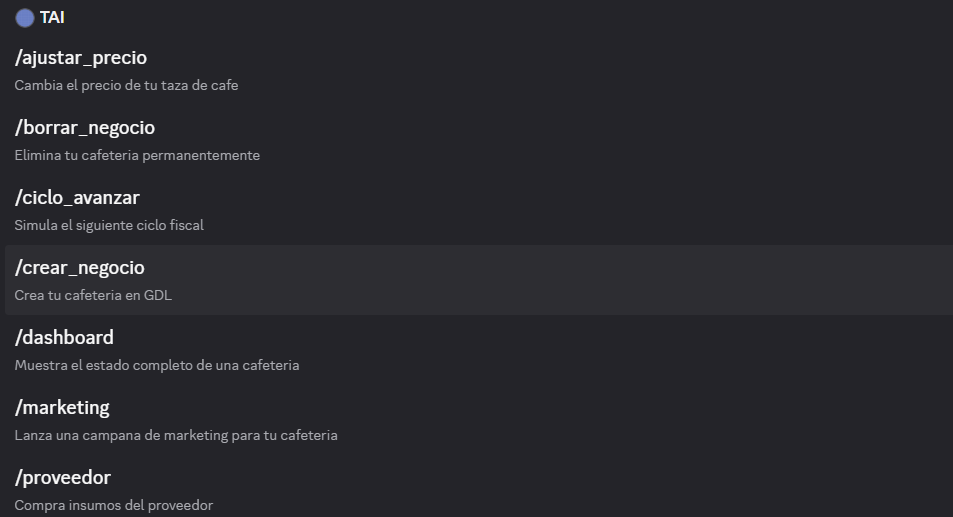
\includegraphics[width=0.75\textwidth]{screenshots/cmd_list.png}}%
  }{%
    \fbox{\parbox{0.75\textwidth}{\centering\vspace{1cm}
    \texttt{[screenshots/cmd\_list.png]}\\\vspace{0.3cm}
    Lista de slash commands del bot TAI en Discord.\vspace{1cm}}}%
  }
  \caption{Todos los slash commands registrados en Discord.}
\end{figure}

\subsection*{7.2 Dashboard -- Estado del negocio}

\begin{figure}[H]
  \centering
  \IfFileExists{screenshots/dashboard.png}{%
    \fbox{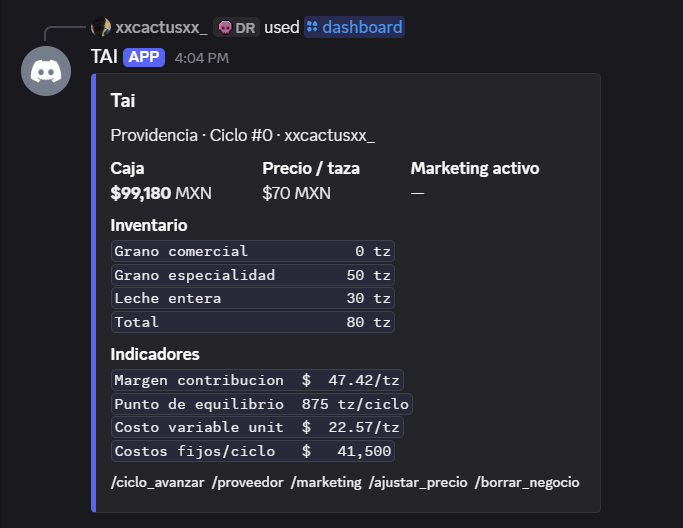
\includegraphics[width=0.85\textwidth]{screenshots/dashboard.png}}%
  }{%
    \fbox{\parbox{0.85\textwidth}{\centering\vspace{1.5cm}
    \texttt{[screenshots/dashboard.png]}\\\vspace{0.3cm}
    Dashboard con caja, inventario, indicadores y ultimo ciclo.\vspace{1.5cm}}}%
  }
  \caption{Embed \texttt{/dashboard} con inventario, indicadores y ultimo ciclo.}
\end{figure}

\subsection*{7.3 Resultado de un ciclo (/ciclo\_avanzar)}

\begin{figure}[H]
  \centering
  \IfFileExists{screenshots/ciclo.png}{%
    \fbox{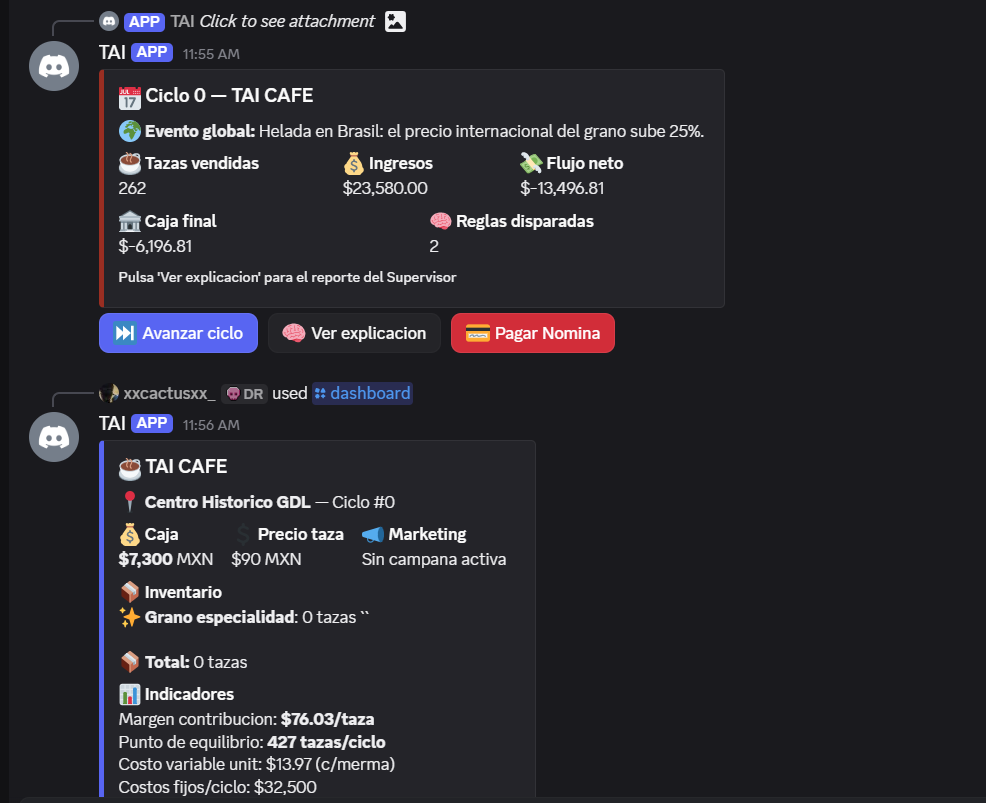
\includegraphics[width=0.85\textwidth]{screenshots/ciclo.png}}%
  }{%
    \fbox{\parbox{0.85\textwidth}{\centering\vspace{1.5cm}
    \texttt{[screenshots/ciclo.png]}\\\vspace{0.3cm}
    Resultado del ciclo: evento global, tazas vendidas, flujo neto, botones.\vspace{1.5cm}}}%
  }
  \caption{Resultado de \texttt{/ciclo\_avanzar} con botones interactivos.}
\end{figure}

% ============================================================
%  8. BASE DE DATOS
% ============================================================
\section{Base de Datos}

Se usa \textbf{SQLite 3} con acceso directo mediante \texttt{sqlite3} de la
biblioteca estándar de Python (sin ORM). El archivo \texttt{se\_discord.db}
se crea automáticamente en la raíz del proyecto.

\subsection*{Tablas}

\begin{center}
\begin{tabular}{>{\bfseries}ll}
  \toprule
  Tabla & Descripción \\
  \midrule
  negocios & Datos maestros del negocio (caja, precio, zona, marketing) \\
  inventario & Tazas equivalentes por tipo de insumo \\
  finanzas\_registro & Histórico de ciclos (ingresos, costos, flujo) \\
  historial\_eventos & Evento global disparado por ciclo \\
  registro\_inferencias & \textbf{Columna vertebral} de la explicabilidad \\
  \bottomrule
\end{tabular}
\end{center}

\subsection*{Diagrama ER simplificado}

\begin{center}
\begin{tikzpicture}[
  ent/.style={draw, rectangle, minimum width=3cm, minimum height=0.7cm,
              align=center, font=\small, fill=accent!10, draw=accent},
  rel/.style={draw, diamond, minimum width=1.5cm, minimum height=0.7cm,
              align=center, font=\tiny, fill=gray!15},
  arr/.style={-},
  node distance=1.6cm and 2.4cm,
]
  \node[ent] (neg) {\textbf{negocios}};
  \node[ent, above right=of neg] (inv) {inventario};
  \node[ent, right=of neg] (fin) {finanzas\_registro};
  \node[ent, below right=of neg] (ev) {historial\_eventos};
  \node[ent, below=of neg] (inf) {registro\_inferencias};

  \draw[arr] (neg) -- node[above,font=\tiny]{1:N} (inv);
  \draw[arr] (neg) -- node[above,font=\tiny]{1:N} (fin);
  \draw[arr] (neg) -- node[above,font=\tiny]{1:N} (ev);
  \draw[arr] (neg) -- node[right,font=\tiny]{1:N} (inf);
\end{tikzpicture}
\end{center}

\subsection*{Tabla \texttt{registro\_inferencias} (explicabilidad)}

\begin{center}
\begin{tabular}{ll}
  \toprule
  Columna & Contenido \\
  \midrule
  \texttt{negocio\_id} & FK a negocios \\
  \texttt{ciclo} & Número del ciclo en que se disparó \\
  \texttt{agente} & \texttt{"pedido"} / \texttt{"atencion"} \\
  \texttt{regla} & Texto de la regla IF-THEN \\
  \texttt{entrada} & Valores que activaron la regla \\
  \texttt{resultado} & Decisión tomada \\
  \texttt{explicacion} & Justificación en lenguaje natural \\
  \bottomrule
\end{tabular}
\end{center}

% ============================================================
%  9. HERRAMIENTAS UTILIZADAS
% ============================================================
\section{Herramientas Utilizadas}

\begin{center}
\begin{tabular}{lll}
  \toprule
  Herramienta & Versión & Uso \\
  \midrule
  Python & 3.11+ & Lenguaje principal \\
  discord.py & 2.x & Framework del bot y UI interactiva \\
  SQLite3 & (stdlib) & Base de datos embebida \\
  LaTeX / MiKTeX & 2024 & Documentación técnica y manual \\
  Git / GitHub & 2.x & Control de versiones y entrega \\
  Discord Developer Portal & -- & Registro del bot y permisos \\
  \bottomrule
\end{tabular}
\end{center}

\subsection*{Fórmulas económicas implementadas}

\begin{tcolorbox}[colback=codebg, colframe=gray!50, fontupper=\small]
\[
  \text{Margen de contribución} = \text{precio} - \text{costo\_variable\_unitario}
\]
\[
  \text{Punto de equilibrio} = \frac{\text{costos\_fijos}}{\text{margen\_contribución}}
\]
\[
  \text{Demanda} = \text{demanda\_base} \times
    \left(\frac{\text{precio\_mercado}}{\text{precio\_usuario}}\right)^{1.5}
\]
\[
  \text{Unidades vendidas} = \min(\text{demanda},\; \text{capacidad},\; \text{inventario})
\]
\[
  \text{Flujo neto} = \text{ingresos} - (\text{costos\_fijos} + \text{costos\_variables})
\]
\end{tcolorbox}

% ============================================================
%  10. CONCLUSIONES
% ============================================================
\section{Conclusiones}

El proyecto \textbf{TAI} demuestra que es viable construir un sistema experto
funcional sobre una plataforma de mensajería como Discord, aprovechando sus
componentes interactivos (buttons, select menus, embeds) como interfaz natural
para un usuario no técnico.

\begin{itemize}
  \item La separación en tres agentes con responsabilidades claras facilita el
        mantenimiento y la extensión del sistema.
  \item El módulo \texttt{registro\_inferencias} hace que el sistema sea
        \textbf{explicable}: el usuario siempre puede saber por qué se tomó
        cada decisión económica.
  \item Las fórmulas puras en \texttt{core/economia.py} son independientes de
        la capa de persistencia, lo que permite probarlas de forma aislada.
  \item El modelo económico con zonas, tipos de insumo y eventos macroeconómicos
        refleja la realidad de operar una cafetería en Guadalajara.
  \item Discord.py facilita el prototipado rápido de interfaces conversacionales
        con componentes gráficos sin necesidad de un frontend web.
\end{itemize}

\newpage

% ============================================================
%  11. MANUAL DE USUARIO
% ============================================================
\section{Manual de Usuario}

\subsection*{11.1 Requisitos previos}

\begin{itemize}
  \item \textbf{Python 3.11 o superior} instalado en el equipo.
  \item \textbf{Cuenta de Discord} y acceso a un servidor donde agregar el bot.
  \item \textbf{Token de bot de Discord} generado en el Developer Portal.
\end{itemize}

\subsection*{11.2 Obtener el token del bot}

\begin{enumerate}
  \item Visita \url{https://discord.com/developers/applications}.
  \item Crea una nueva aplicación o selecciona la existente.
  \item En el menú lateral, ve a \textbf{Bot}.
  \item Activa \textbf{Message Content Intent} en ``Privileged Gateway Intents''.
  \item Copia el token con el botón \textbf{Reset Token}.
\end{enumerate}

\subsection*{11.3 Instalación}

\begin{lstlisting}[style=python, language={}]
# 1. Clona el repositorio
git clone https://github.com/<usuario>/SE-Discord.git
cd SE-Discord

# 2. (Recomendado) Crea un entorno virtual
python -m venv .venv

# Windows:
.venv\Scripts\activate
# Linux / macOS:
source .venv/bin/activate

# 3. Instala dependencias
pip install -r requirements.txt
\end{lstlisting}

El archivo \texttt{requirements.txt} contiene:
\begin{lstlisting}[style=python, language={}]
discord.py>=2.3.0
\end{lstlisting}

\subsection*{11.4 Configuración del token}

\begin{lstlisting}[style=python, language={}]
# Windows (PowerShell)
$env:DISCORD_TOKEN = "tu_token_aqui"

# Linux / macOS
export DISCORD_TOKEN="tu_token_aqui"
\end{lstlisting}

\textbf{Importante:} nunca subas el token al repositorio.

\subsection*{11.5 Ejecutar el bot}

\begin{lstlisting}[style=python, language={}]
python bot.py
\end{lstlisting}

Si todo está correcto verás en la consola:
\begin{lstlisting}[style=python, language={}]
Conectado como TAI#7626  -  comandos sincronizados
\end{lstlisting}

La primera vez se crea automáticamente \texttt{se\_discord.db} con las
cinco tablas del esquema.

\subsection*{11.6 Invitar el bot a tu servidor}

\begin{enumerate}
  \item En el Developer Portal, ve a \textbf{OAuth2 > URL Generator}.
  \item Selecciona los scopes \texttt{bot} y \texttt{applications.commands}.
  \item En Bot Permissions activa: \textit{Send Messages}, \textit{Use Slash Commands},
        \textit{Embed Links}, \textit{Read Message History}.
  \item Copia la URL generada, pégala en el navegador e invita el bot.
\end{enumerate}

\subsection*{11.7 Guía de uso — Comandos}

\subsubsection*{/crear\_negocio}

Crea tu cafetería. Debes proporcionar:
\begin{itemize}
  \item \texttt{nombre} — nombre de tu cafetería.
  \item \texttt{zona} — elige una de las 6 zonas de la ZMG del selector.
\end{itemize}

El sistema asigna caja inicial de \$100,000 MXN, precio de \$55/taza
e inventario inicial de 100 tazas (grano comercial) + 60 tazas (leche).

\subsubsection*{/dashboard}

Muestra el estado completo:
\begin{itemize}
  \item Caja actual, precio por taza y bonus de marketing activo.
  \item Inventario desglosado por tipo de insumo.
  \item Resultados del último ciclo (ingresos, costos, flujo neto).
  \item Indicadores: margen de contribución, punto de equilibrio,
        costo variable unitario y costos fijos del ciclo.
\end{itemize}

Si hay más de una cafetería en el servidor, aparece un selector para elegir cuál ver.

\subsubsection*{/ciclo\_avanzar}

Simula un mes fiscal completo:
\begin{enumerate}
  \item Se genera un evento macroeconómico aleatorio.
  \item El motor de reglas evalúa el estado del negocio.
  \item Se calcula demanda, ventas, costos y flujo neto.
  \item Se persisten resultados en la base de datos.
  \item Se consume el inventario (con merma del 7.5\,\%).
  \item El bonus de marketing decae al 50\,\%.
\end{enumerate}

Aparecen cuatro botones:
\begin{itemize}
  \item \textbf{Avanzar ciclo} — repite el ciclo sin escribir el comando.
  \item \textbf{Ver explicación} — muestra el reporte del Agente Supervisor.
  \item \textbf{Vender} — venta rápida proporcional a la demanda actual.
  \item \textbf{Pagar Nómina} — descuenta \$8,500 MXN de la caja manualmente.
\end{itemize}

\subsubsection*{/proveedor}

Abre un Select Menu para comprar insumos:

\begin{center}
\begin{tabular}{llrr}
  \toprule
  Insumo & Calidad & Costo & Tazas \\
  \midrule
  Grano comercial & Media & \$300 & +50 \\
  Grano especialidad & Alta (Chiapas/Veracruz) & \$700 & +50 \\
  Leche entera & Base & \$120 & +30 \\
  Alternativa vegetal & Avena/almendra & \$270 & +30 \\
  \bottomrule
\end{tabular}
\end{center}

\subsubsection*{/marketing}

Lanza una campaña que eleva la demanda base temporalmente:

\begin{center}
\begin{tabular}{llrr}
  \toprule
  Campaña & Bonus demanda & Costo & Decaimiento \\
  \midrule
  Redes sociales & +10\,\% & \$3,000 & 50\,\%/ciclo \\
  Influencer & +20\,\% & \$8,000 & 50\,\%/ciclo \\
  Descuento apertura & +25\,\% & \$1,500 & 50\,\%/ciclo \\
  Cata en tienda & +15\,\% & \$5,000 & 50\,\%/ciclo \\
  \bottomrule
\end{tabular}
\end{center}

\subsubsection*{/ajustar\_precio}

Cambia el precio por taza. El sistema advierte si el precio está
más de \$10 por encima o por debajo del precio de mercado (\$55 MXN).

\subsubsection*{/borrar\_negocio}

Elimina permanentemente la cafetería con todos sus datos (inventario,
historial, finanzas e inferencias). Requiere confirmación con un botón.

\subsection*{11.8 Interpretar el Dashboard}

\begin{itemize}
  \item \textbf{Color del embed:} verde = flujo positivo, amarillo = pérdida leve
        ($< \$5{,}000$), rojo = pérdida mayor, gris azul = sin ciclos.
  \item \textbf{Margen de contribución:} si es negativo, cada taza vendida genera
        pérdida. Sube el precio o baja el costo de insumo.
  \item \textbf{Punto de equilibrio:} número mínimo de tazas que debes vender para
        no perder dinero. Compara con las tazas vendidas del último ciclo.
\end{itemize}

\subsection*{11.9 Estrategias recomendadas}

\begin{enumerate}
  \item \textbf{Inicio:} compra grano comercial + leche. Precio \$55. Avanza ciclos.
  \item \textbf{Crecimiento:} cuando la caja supere \$30,000, compra grano de
        especialidad para activar el bono de reputación (+15\,\% demanda).
  \item \textbf{Marketing:} con caja sólida, lanza ``Descuento apertura'' (\$1,500,
        +25\,\%) para maximizar ventas un ciclo.
  \item \textbf{Ajuste de precio:} si la regla ``Precio alto'' se dispara
        repetidamente, baja el precio o compensa con calidad/marketing.
  \item \textbf{Zona premium:} Andares ofrece la mayor renta (×1.8) pero también
        demanda alta (×1.1); es rentable solo con precio y calidad altos.
\end{enumerate}

\subsection*{11.10 Preguntas frecuentes}

\begin{description}
  \item[El bot no responde a los comandos slash.]
    Asegúrate de que el bot tenga el permiso \texttt{applications.commands}
    y de que los slash commands se hayan sincronizado (\texttt{on\_ready}
    llama a \texttt{bot.tree.sync()}).

  \item[La caja se fue a negativo.]
    El simulador permite saldo negativo para reflejar deuda real.
    Usa \texttt{/proveedor} para reabastecerte y avanza ciclos con mayor precio.

  \item[¿Cómo reiniciar mi cafetería?]
    Usa \texttt{/borrar\_negocio} y luego \texttt{/crear\_negocio} con los
    nuevos parámetros.

  \item[¿Qué pasa si el inventario llega a cero?]
    El ciclo venderá 0 tazas. El flujo neto será negativo por los costos fijos.
    Usa \texttt{/proveedor} antes de avanzar el siguiente ciclo.
\end{description}

\end{document}
